\documentclass[a4paper,12pt]{article} 


\usepackage[T2A]{fontenc}			% кодировка
\usepackage[utf8]{inputenc}			% кодировка исходного текста
\usepackage[english,russian]{babel}	% локализация и переносы


% Математика
\usepackage{amsmath,amsfonts,amssymb,amsthm,mathtools} 

\usepackage{gensymb}	
\usepackage{wasysym}

% Картинки
\usepackage{graphicx}
\graphicspath{{images/}}
\usepackage{rotating}

%Заговолок
\usepackage[left=2cm,right=2cm,
    top=2cm,bottom=2cm,bindingoffset=0cm]{geometry}

\usepackage{titling}


\author{Петров Артём Антонович, группа 721}
\title{Лабораторная работа № 123 "Резонанс токов в параллельном контуре"}
\date{\today}

\begin{document} % начало документа

\begin{minipage}[t][7cm]{\textwidth}
\maketitle
\end{minipage}


\textbf{Цель работы:} исследование резонанса токов в параллельном колебательном контуре с изменяемой ёмкостью, включающее получение амплитудно-частотных и фазово-частотных характеристик, а также
определение основных параметров контура.
\bigskip

\medskip
\textbf{Оборудование:} генератор сигналов, источник тока, нагруженный на параллельный колебательный
контур с переменной ёмкостью, двулучевой осциллограф, цифровые вольтметры.

\bigskip


\subsection*{Экспериментальная установка}
\bigskip


\begin{figure}[ht]
\centering
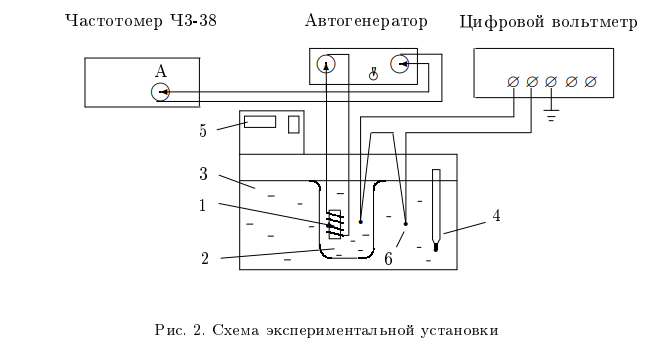
\includegraphics[width=80mm]{scheme.png}
\caption{Схема установки: Колебательный контур $L-C_n-R$, где паразитное сопротивление $R_L$ отвечает за собственное сопротивление катушки. }\label{schema}
\end{figure}

\bigskip

\subsection*{Ход работы}
\bigskip

В нашем эксперименте мы изучали резонанс колебательного контура. Полученная зависимость резонансной частоты контура $f_0$ от величины питающего напряжения $E$ и напряжения на эталонном резисторе $R_1$ $U$, а также всевозможные параметры колебательного контура, полученные на основе этих измерений представлены в таблице \ref{table1} . В том числе столь интересующие нас значения индуктивности катушки $L$ и её активного сопротивления $R_L$.

Также для значений $C_n$ номер 2 и 6 были получены АЧХ и ФЧХ, представленные на графиках \ref{achh1}, \ref{achh2} и \ref{fchh1}.

По графику АЧХ (график \ref{achh1}) видно, что при резонансе, соответствующему ёмкости $C_2$ напряжение достигает более высоких значений, чем при ёмкости $C_6$, что соответствует более высокой добротности контура при значении ёмкости равном $С_2$ (что подтверждается данными из таблицы \ref{table1}).
 
При переходе в безразмерные координаты (график \ref{achh2}) можно легко оценить добротность по ширине резонансных кривых на уровне $\frac{U}{U_0} = \frac{1}{\sqrt{2}}$.

\bigskip
Полученная оценка: 

\bigskip

Что сходится с данными из таблицы \ref{table1}.

По ФЧХ (график \ref{fchh1}) можно оценить добротность иным способом: расстоянию между точками по оси $f/f_0$, в которых $\phi_U/\pi$ меняется от $-\pi/4$ до $\pi/4$. Это расстояние равно $1/Q$.

\bigskip
Полученная оценка:

\bigskip

Что сходится с данными из таблицы \ref{table1}.

\bigskip

\bigskip

\bigskip

По графику зависимости $R_L(F_{0n})$ видно, что $R_L$ отнюдь не постоянно при различных частотах, как этого можно было бы ожидать при предположении, что $R_L$ определяется сугубо собственным сопротивлением проводов катушки индуктивности. Видно, что $R_L$ растёт с ростом частоты $f_0$. Это можно попробовать объяснить тем, что в $R_L$ вносят вклад затраты энергии на перемагничивание сердечника катушки при смене направления тока в ней. Ведь, чем выше частота $f_0$, тем чаще нужно перемагничивать сердечник и тем больше потери энергии в единицу времени, а значит, и больше $R_L$.





\begin{sidewaysfigure}[ht]
\centering
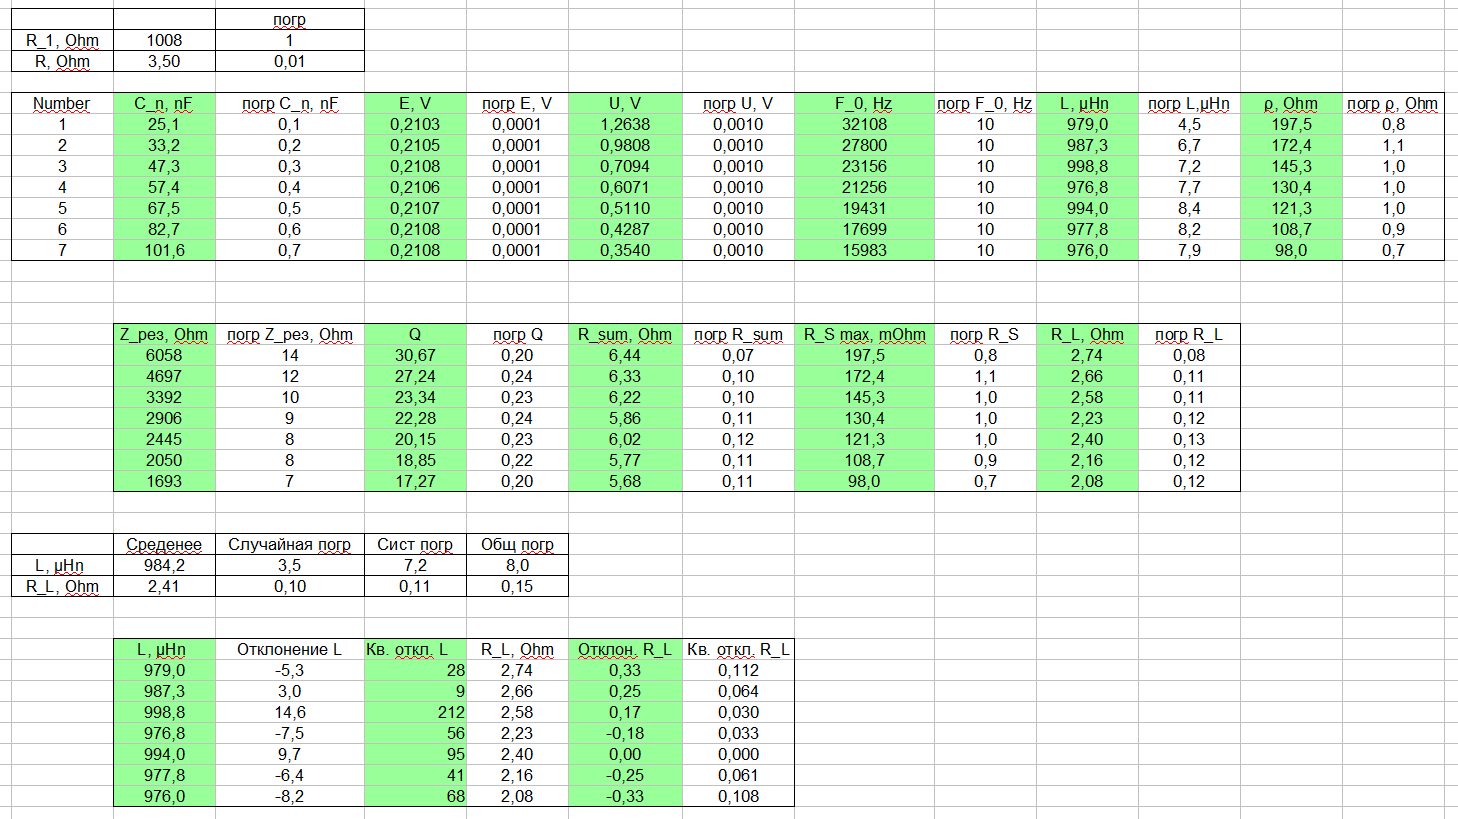
\includegraphics[width=220mm]{table_final.png}
\caption{Таблица значений различных параметров колебательного контура при разных $C_n$ и их погрешностей.}\label{table1}
\end{sidewaysfigure}

\begin{figure}[ht]
\centering
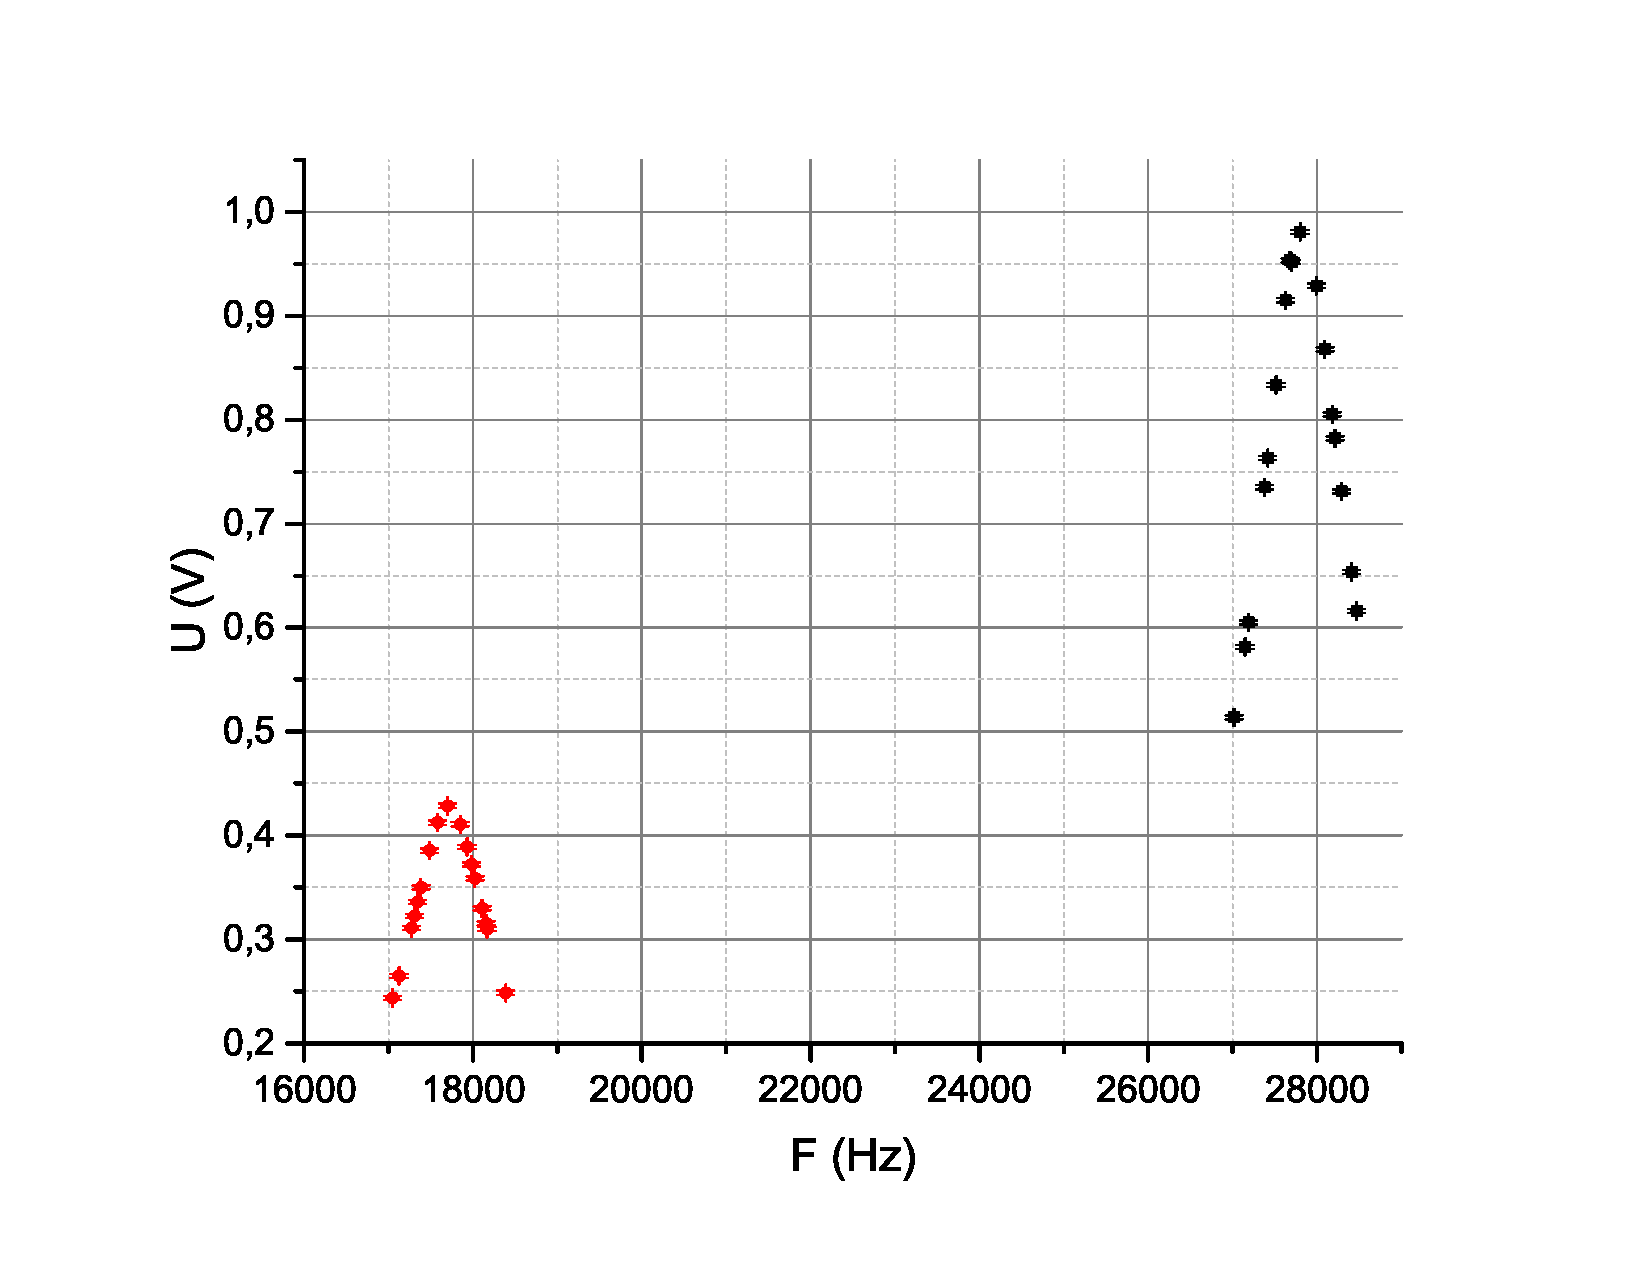
\includegraphics[width=150mm]{graph12.eps}
\caption{АЧХ для контуров номер 2(справа) и 6(слева)}\label{achh1}
\end{figure}

\begin{figure}[ht]
\centering
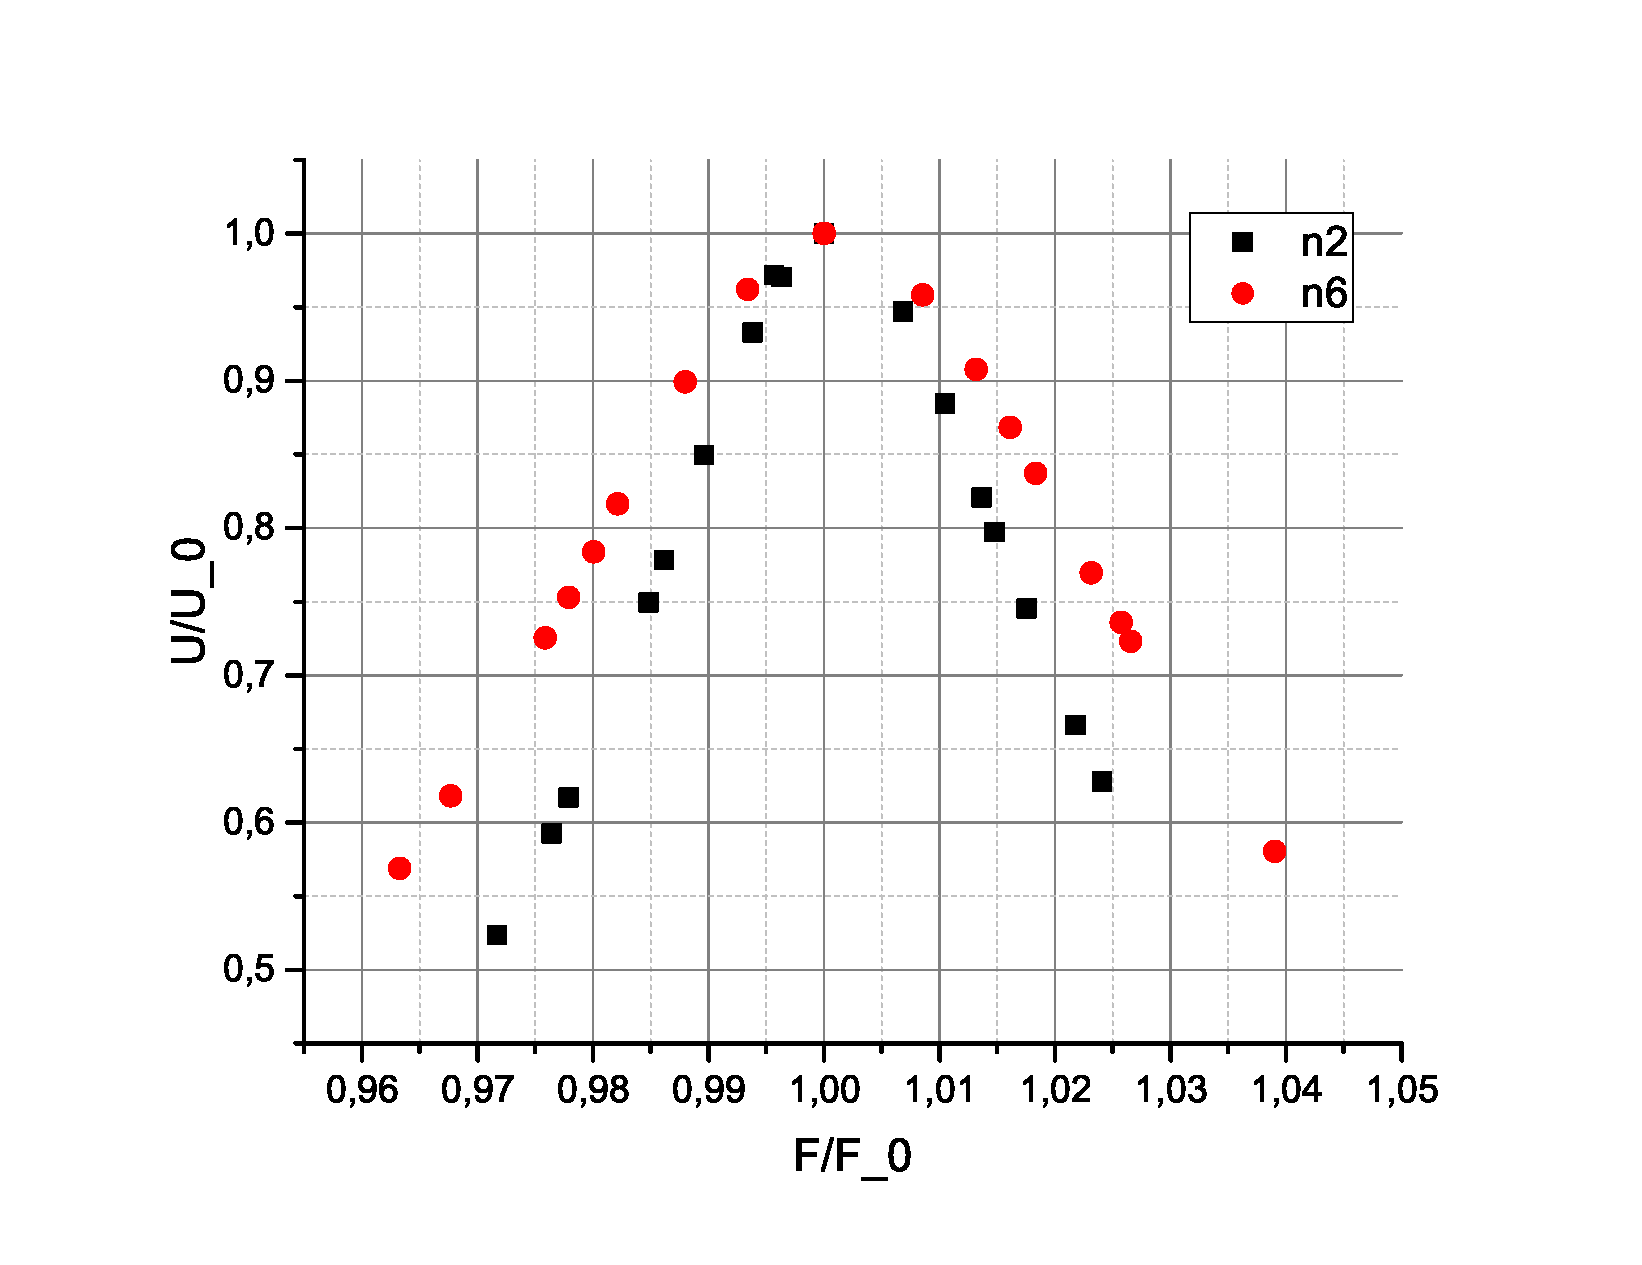
\includegraphics[width=150mm]{graph13.eps}
\caption{АЧХ для контуров номер 2 и 6 в безразмерных координатах ($U/U_0$ от $f/f_0$). }\label{achh2}
\end{figure}

\begin{figure}[ht]
\centering
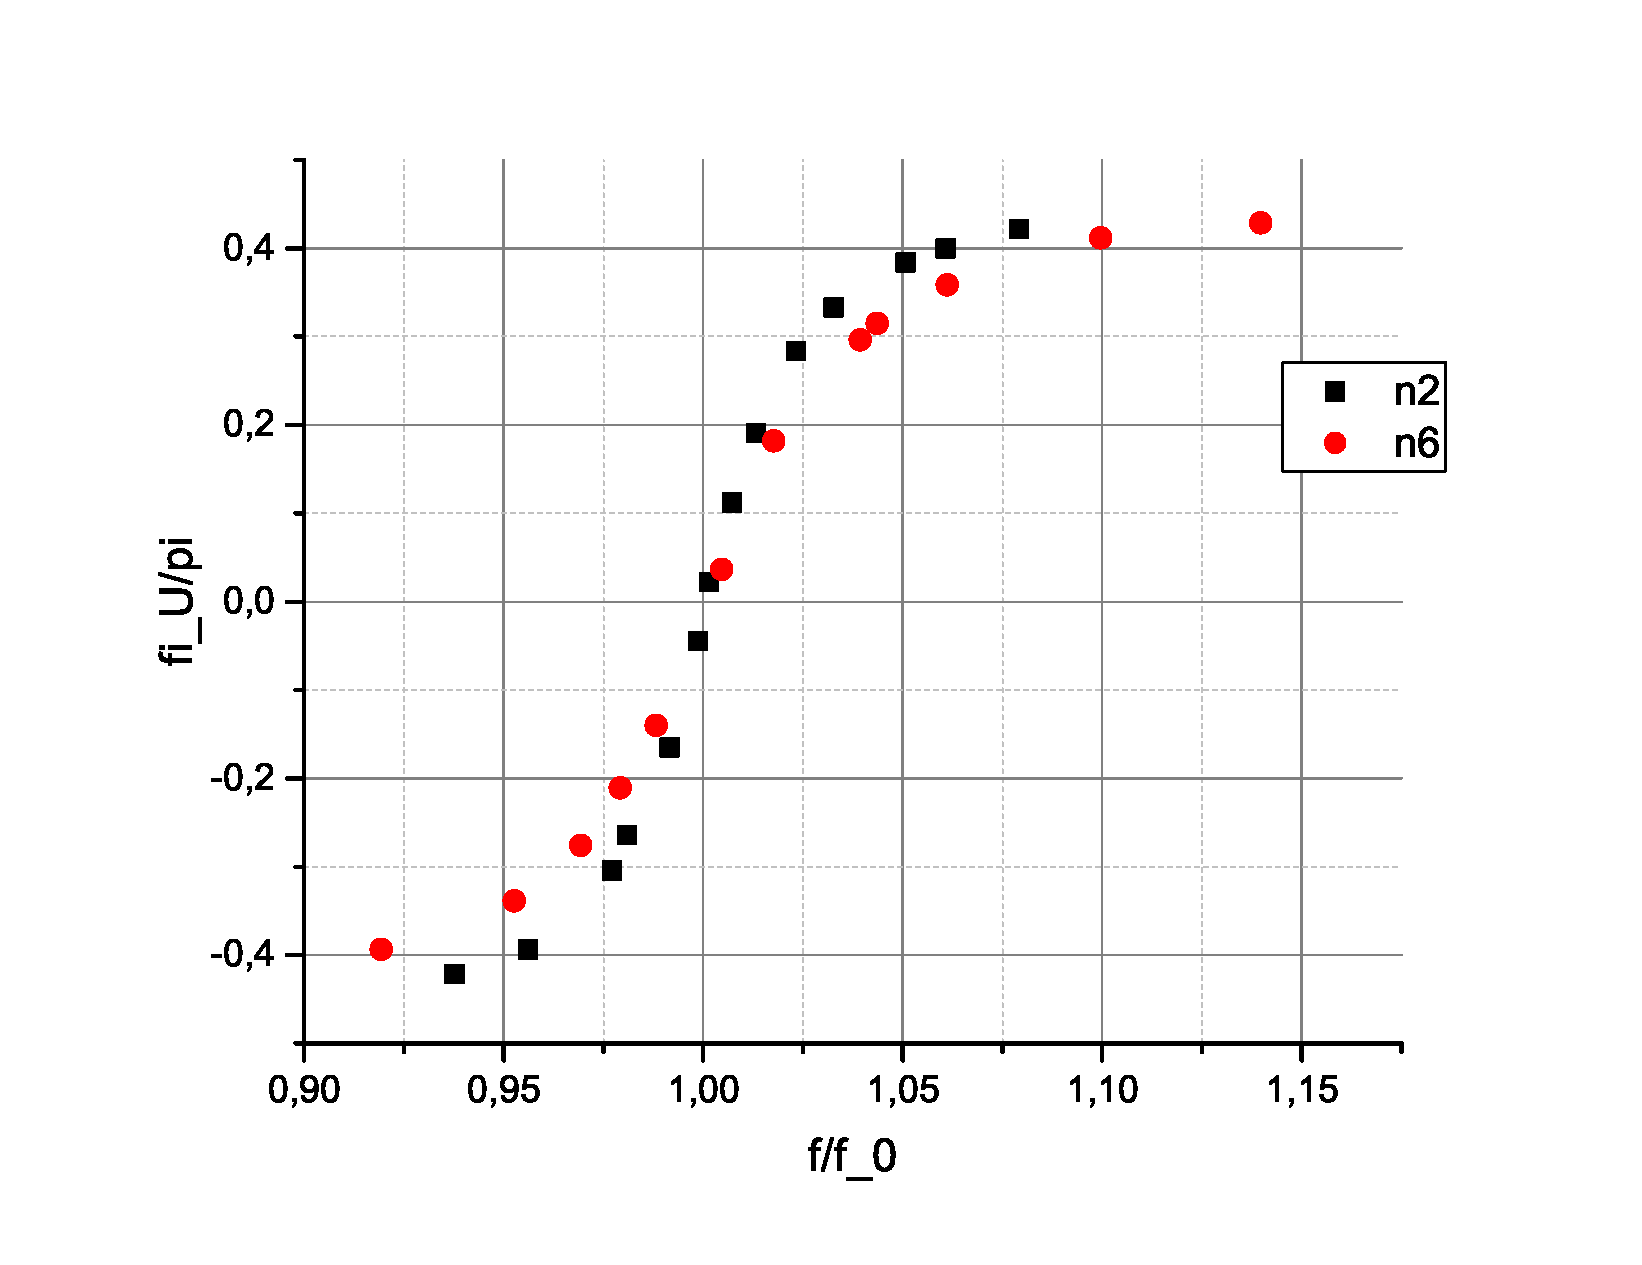
\includegraphics[width=150mm]{graph14.eps}
\caption{ФЧХ для контуров номер 2 и 6 в безразмерных координатах ($\phi_U/\pi$ от $f/f_0$).}\label{fchh1}
\end{figure}

\begin{figure}[ht]
\centering
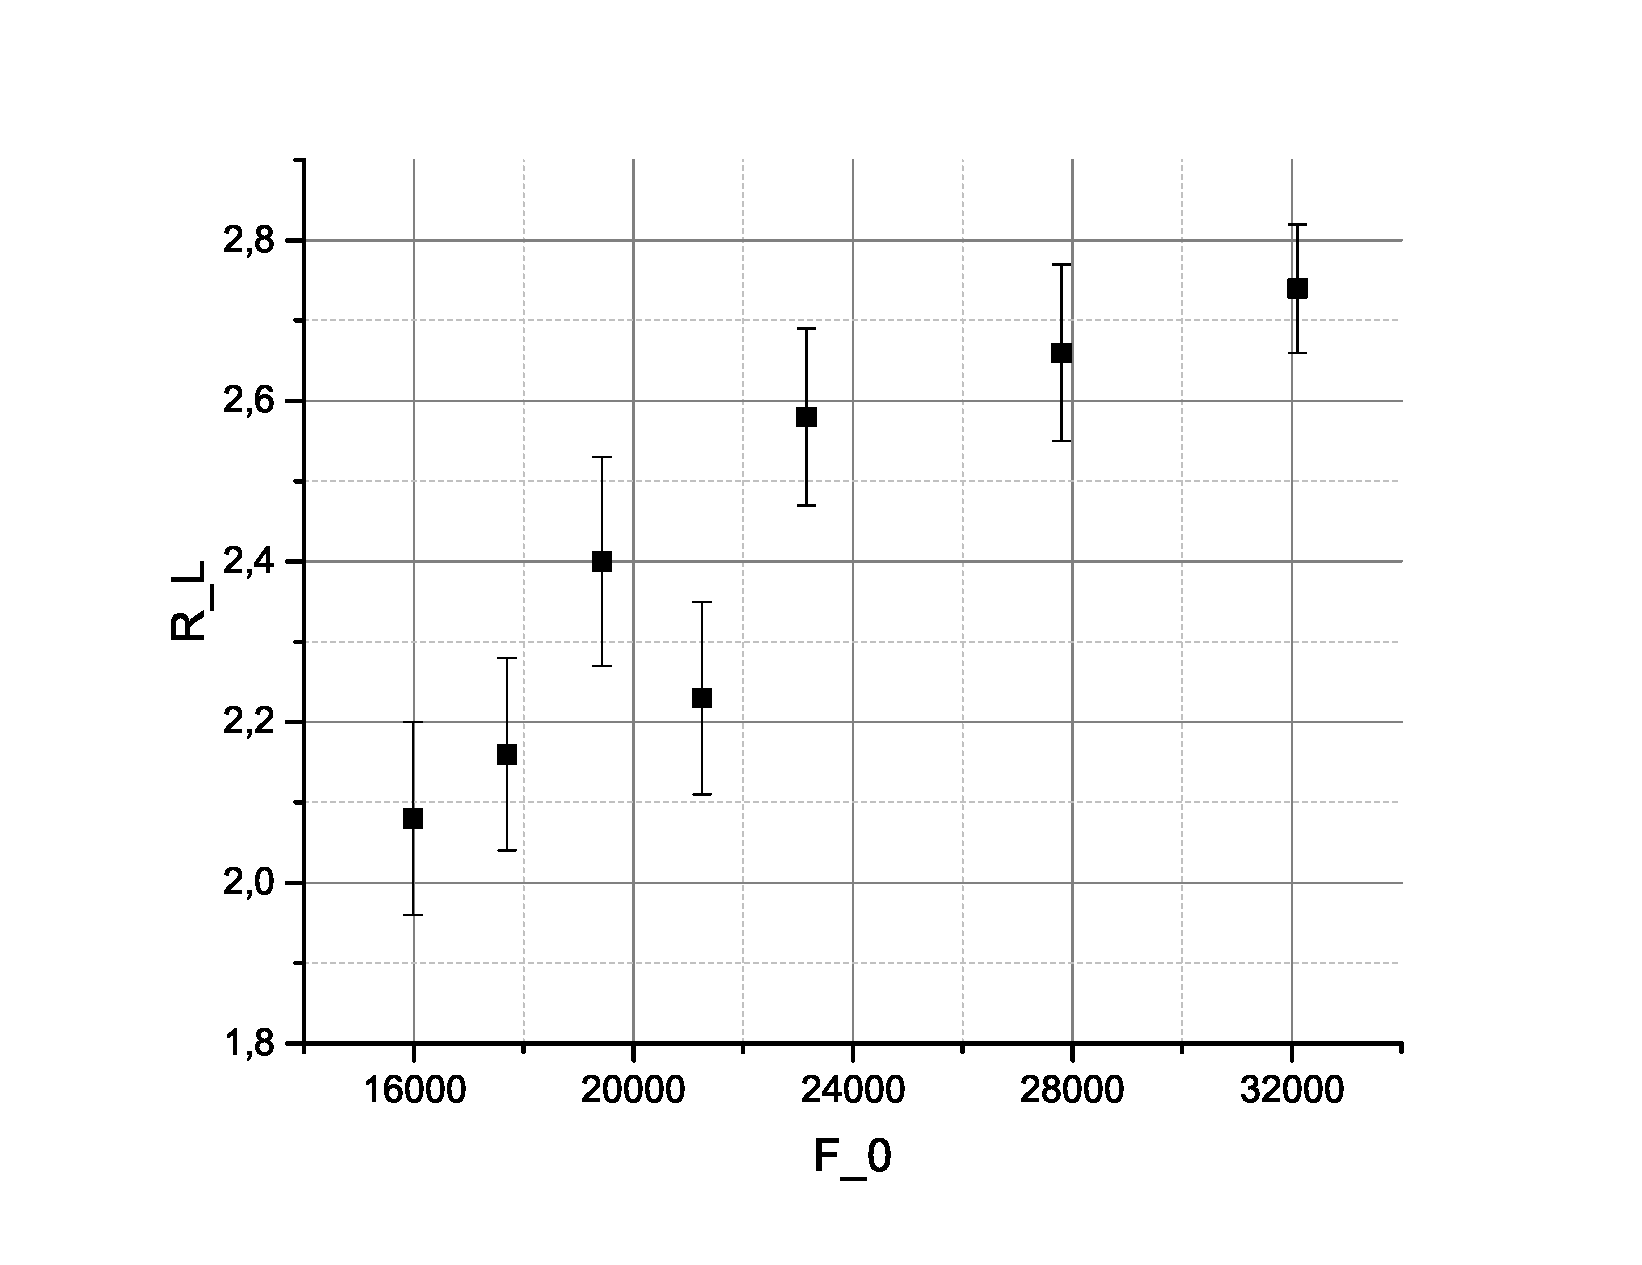
\includegraphics[width=150mm]{graph15.eps}
\caption{Зависимость $R_L$ от резонансной частоты для разных значений $C_n$]}\label{plotrl}
\end{figure}


\bigskip

\textbf{Итог:}
\bigskip
 
\end{document} % конец документа